\documentclass[13pt, t]{beamer}
% Presento style file
\usepackage{config/presento}

% custom command and packages
% custom packages
\usepackage{textpos}
\setlength{\TPHorizModule}{1cm}
\setlength{\TPVertModule}{1cm}

\newcommand\crule[1][black]{\textcolor{#1}{\rule{2cm}{2cm}}}



\usepackage{color, colortbl}

\title{\Large \hspace{-0.5cm} Analysing phonological systems: \\ on Bayesian typological research}
\author[shortname]{George Moroz}
\institute[shortinst]{Linguistic Convergence Laboratory, NRU HSE, Moscow, Russia}
\date{\begin{center} 24 August 2019 \bigskip \\ Societas Linguistica Europaea, 52nd Annual Meeting, Leipzig University\\ \vfill Presentation is available here: {\large \href{https://tinyurl.com/y3wtkcbq}{tinyurl.com/y3wtkcbq} \hfill 
\includegraphics[height = 2.5cm]{images/01_qrcode}} \end{center}}

\begin{document}

\begin{frame}[plain]
\maketitle
\end{frame}

\begin{frame}{In this talk I will cover the following:}
\begin{itemize}
\item goals of the linguistic typology
\item different strategies of sampling
\item Bayesian way of thinking about the linguistic typology
\item Case study: vowels
\end{itemize}
\end{frame}

\begin{frame}{Goals of the linguistic typology}
\begin{itemize}
\item attest distributions (statistical and areal) of typological values \pause
\item find a correlation of distributions of different typological categories
\begin{itemize}
\item absolute universals
\item distributional patterns and tendencies
\item semantic maps
\item diachronic change of typological values \pause
\end{itemize}
\item find a correlation of linguistic and non-linguistic patterns
\begin{itemize}
\item population movements
\item population size
\item language contact
\item sociolinguistic parameters
\item geopolitical environment (including diseases' spread) \pause
\end{itemize}
\item deal with a mixed typological value per language
\end{itemize}
\end{frame}

\begin{frame}{Frequentist typological research}
\begin{itemize}
\item Formulate a theoretical question\\
There is a category in some languages with values \textbf{VAL 1} and \textbf{VAL 2}. \pause \\
What is the probability $\theta$ to meet \textbf{VAL 1} in randomly picked language? \pause
\item[◌] Get a grant, hire some students, or select a holiday, which you want to spent working on this topic... \pause
\item Pick a sample of languages, calculate desired statistics, e. g. $\hat{\theta}$ \pause
\item From now $\hat{\theta}$ is the best estimation of $\theta$ that you know\pause, if you want to convince a mad about statistics editor, add some \textbf{confidence intervals}
\item[◌] After you published your paper project is finished
\end{itemize}
\end{frame}

\begin{frame}{There are different type of sampling}
\begin{multicols}{2}
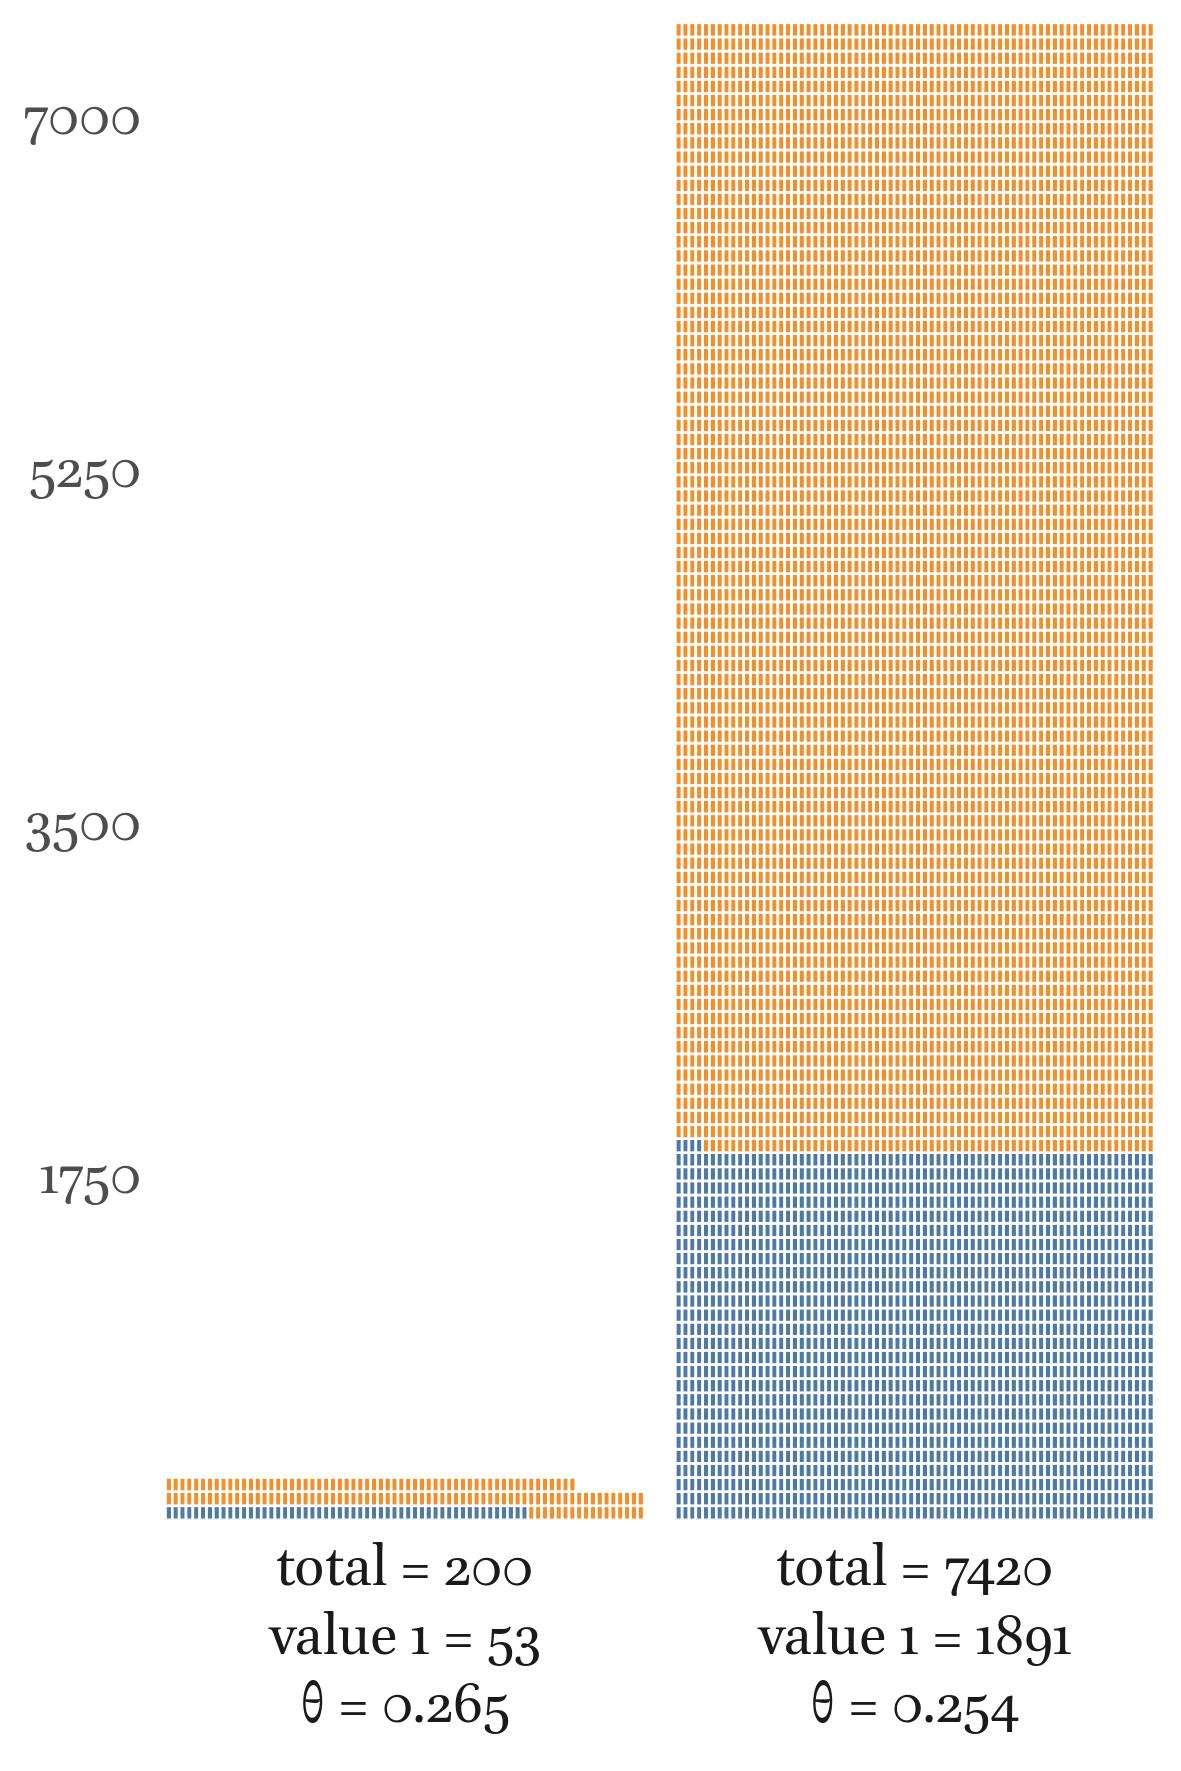
\includegraphics[width=\linewidth]{images/03_simple_sample}
\columnbreak

\textbf{Random sampling:}\\
each element in the population has an equal probability of selection \pause\\
\begin{itemize}
\item[\color{colorblue}!!!] but each language is grouped in \textbf{a language family} and \textbf{an area}, so each observation is not independent\dots
\end{itemize}

\end{multicols}
\end{frame}

\begin{frame}{Language families (languages > 10)}
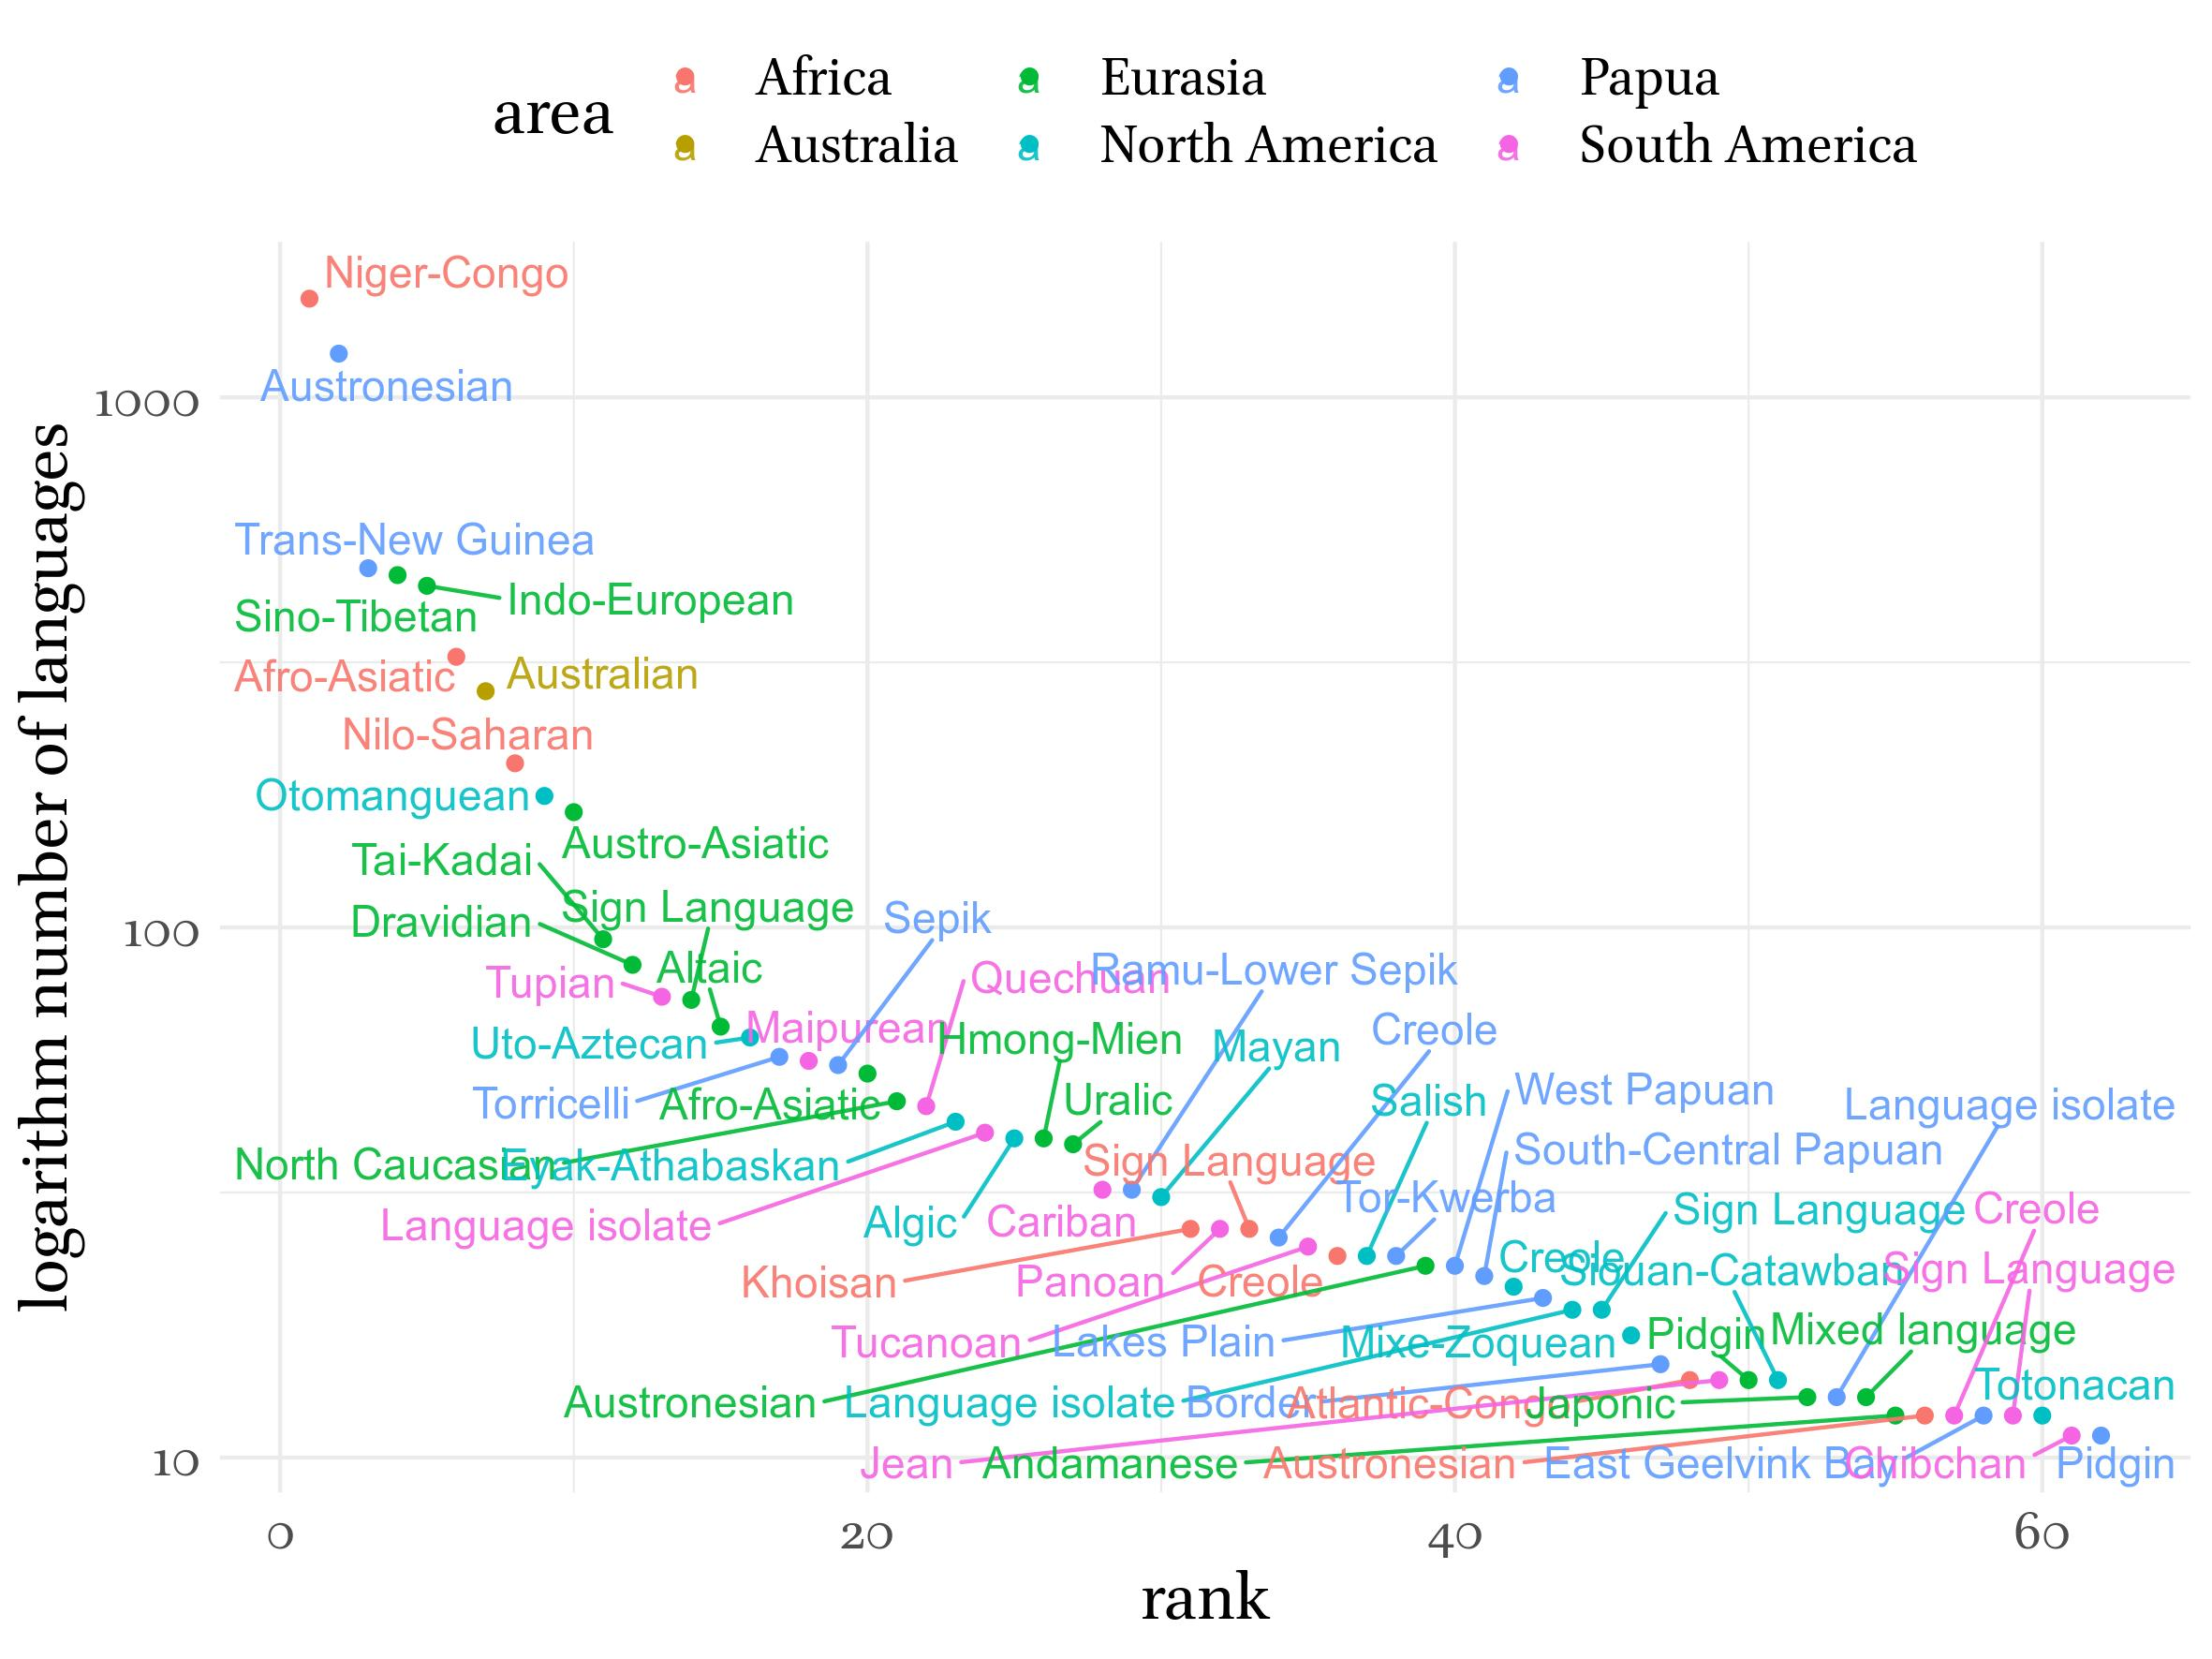
\includegraphics[width=\linewidth]{images/04_families_by_area}
\end{frame}

\begin{frame}{There are different type of sampling:}
\begin{multicols}{2}
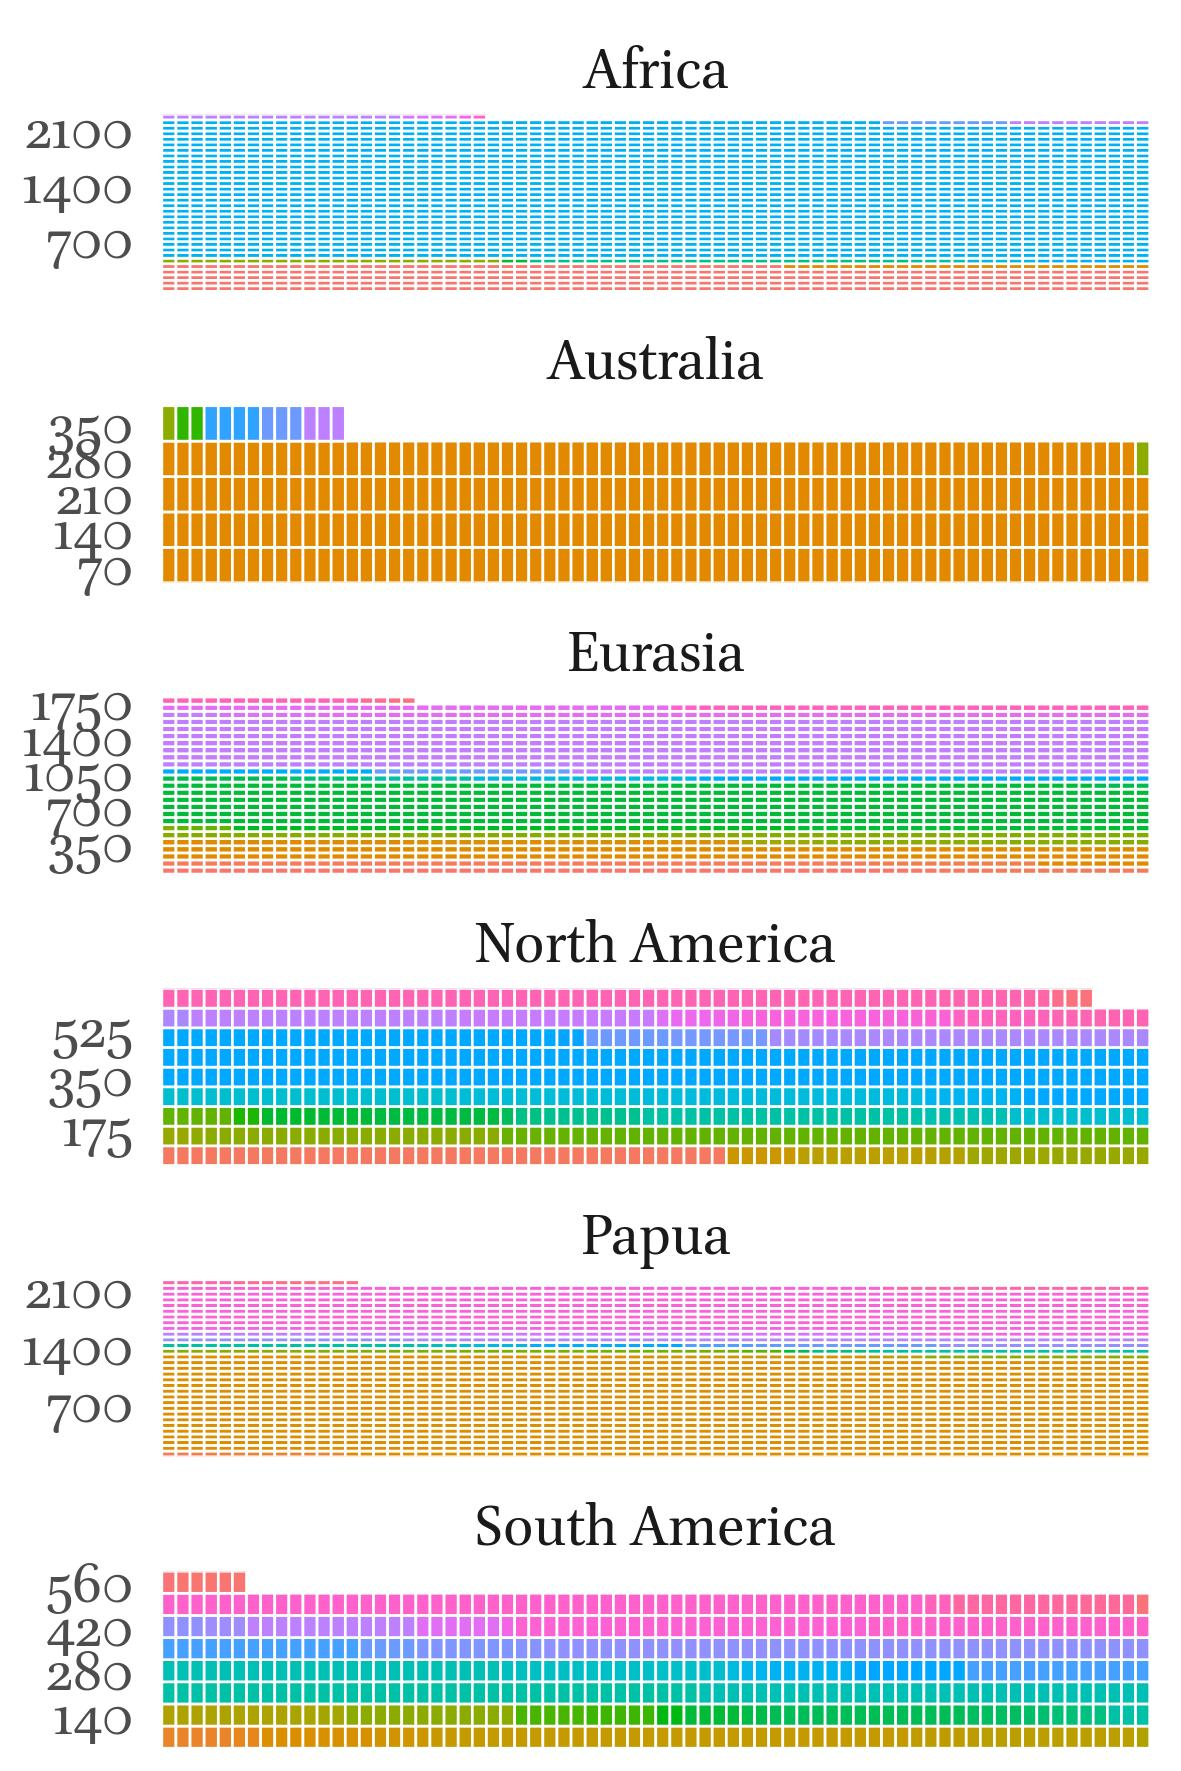
\includegraphics[width=\linewidth]{images/05_families_by_area}
\columnbreak

\textbf{Stratified random sampling}\\
divide population into groups that differ in important ways and then perform random sampling from each group\pause\\
\begin{itemize}
\item[\color{colorblue}!!!] The Glottolog version in the \texttt{\small lingtypology} package suggests that there are \\ \alert{214 unique combinations} (142 sign languages and 82 isolates counted as one family) \pause
\item[\color{colorblue}$\Rightarrow$] So for creating statistically reasonable sample one need to get around 300 languages
\end{itemize}
\end{multicols}
\end{frame}

\begin{frame}{I am not the first}
\begin{itemize}
\item \citep{bell78} "Language Samples"
\item \citep{dryer89} "Large Linguistic Areas and Language Sampling"
\item \citep{perkins89} "Statistical Techniques for Determining Language Sample Size"
\item \citep{nichols92} "Linguistic Diversity in Space and Time"
\item \citep{rietveld93} "Statistical Techniques for the Study of Language and Language Behaviour"
\item \citep{rijkhoff98} "Language sampling"
\item \citep{maslova00} "A dynamic approach to the verification of distributional universals"
\item \citep{widmann01} "Language Sampling for Typological Studies"
\item \citep{janssen06} "Randomization Tests in Language Typology"
\item \citep{bakker10} "Language Sampling"
\end{itemize}
\end{frame}

\begin{frame}{What about phonology?}
It is possible to use phonological units or relation of any phonological theory you like:
\begin{itemize}
\item features, feet, syllables, etc.
\item feature constituents, OT constraints, exemplars, phonological alternations
\item phonological distinctions (e. g. /i/ vs. /ɨ/)
\item ...
\end{itemize}
\end{frame}

\framecard[colorblue]{{\color{colorwhite} \Large Send me a letter!\\
agricolamzgmail.com\\ 
\vfill Presentation is available here: \\tinyurl.com/y3wtkcbq\\
\vfill  
\includegraphics[height = 4cm]{images/02_qrcode}}}

\begin{frame}{References}
\footnotesize
\bibliographystyle{config/chicago}
\bibliography{bibliography}
\end{frame}

\end{document}